%%%%%%%%%% Recovery Algorithms Descriptions %%%%%%%%%%%%%%%%%%
\section{Recovery Algorithms}
\label{sec:algs}

In this section we propose three new recovery algorithms: \seconds, \purges, and \cprs.  
%Although recovery is implemented differently across these algorithms, the input and output of each algorithm is the same.
With one exception, the input and output of each algorithm is the same. 
{\footnote {\small Additionally, as input \cpr requires that each $v \in adj($\bads$)$ is notified of the time, $t'$, in which \bad was compromised.}}
\begin{itemize}
	\item {\bf Input:}  Undirected graph, $G=(V,E)$, with weight function $w: E \rightarrow \mathbb{N}$.  $\forall v \in V$,  \minvv and \dmatrixv are computed
(using distance vector). Also, each $v \in adj($\bads$)$ is notified that \bad was compromised.

	\item {\bf Output:} Undirected graph, $G'=(V',E')$, where $V' = V -\{$\bads$\}$, $E'=E - \{(\bar{v},v_i)$ $|$ $v_i \in adj(\bar{v}) \}$,
%(adj(\bar{v}),\bar{v})$ $\forall adj(\bar{v})$,
and link weight function $w:E \rightarrow \mathbb{N}$.  \minvv and \dmatrixv are computed via the algorithms discussed below $\forall  v \in V'$. 
\end{itemize}
Before we describe each recovery algorithm, we outline a preprocessing procedure common to all three recovery algorithms.
%First we describe a preprocessing procedure common to all three recovery algorithms. Then we describe each recovery algorithm. 


\subsection{Preprocessing}
\label{subsec:preprocess}
All three recovery algorithms share a common preprocessing procedure.  The procedure removes \bad as a destination and finds the node IDs in each connected component. 
This is implemented using diffusing computations \cite{Dijkstra80} initiated at each $v \in adj($\bads$)$. 
A diffusing computation is a distributed algorithm started at a source
node which grows by sending queries along a spanning tree, constructed
simultaneously as the queries propagate through the network.  When the computation reaches the leaves
of the spanning tree, replies travel back along the tree towards the
source, causing the tree to shrink. The computation eventually terminates when the
source receives replies from each of its children in the tree. 

In our case, each diffusing computation message contains a vector of node IDs.  When 
a node receives a diffusing computation message, the node adds its ID to the vector and removes \bad as a destination. At the end of the diffusing computation, 
each $v \in adj($\bads$)$ has a vector that includes all nodes in $v$'s connected component. Finally, each $v \in adj($\bads$)$ broadcasts the vector of node IDs to 
all nodes in their connected component. In the case where removing \bad partitions the network, each node will only compute shortest paths to nodes in the vector. 

Consider the example in Figure \ref{fig:dv-example} where \bad is the compromised node. 
When $i$ receives the notification that \bad has been compromised, $i$ removes \bad as a destination and then initiates a diffusing computation. 
$i$ creates a vector and adds its node ID to the vector. $i$ sends a message containing this vector to $j$ and $k$.  Upon receiving $i$'s message,
$j$ and $k$ both remove \bad as a destination and add their own ID to the message's vector.  Finally, $l$ and $d$ receive a message from $j$ and $k$, respectively.  
$l$ and $d$ add their node own ID to the message's vector and remove \bad as a destination. Then, $l$ and $d$ send an ACK message back to $j$ and $k$, respectively, with the complete 
list of node IDs. Eventually when $i$ receives the ACKs from $j$ and $k$, $i$ has a complete list of nodes in its connected component. Finally, $i$ broadcasts the vector of node IDs
in its connected component. 

%In this example, the graph remains connected after removing \bads.   

\subsection{The 2$^{nd}$ best Algorithm}
\label{subsec:second}
%\second is a simple extension to distance vector which provides correct recovery from compromised nodes.
\second invalidates state locally and then uses distance vector to implement network-wide recovery.  Following the preprocessing described in Section \ref{subsec:preprocess}, 
each neighbor of the compromised node locally invalidates state by selecting the least cost pre-existing alternate path that does not use the compromised node as the first hop.
The resulting distance vectors trigger the execution of traditional distance vector to remove the remaining false state.
Algorithm \ref{alg:second} in the Appendix gives a complete specification of \seconds.

\begin{figure*}[t]
  \begin{center}
    \subfigure[Before $\overline{v}$ is compromised.]{\label{fig:example-a}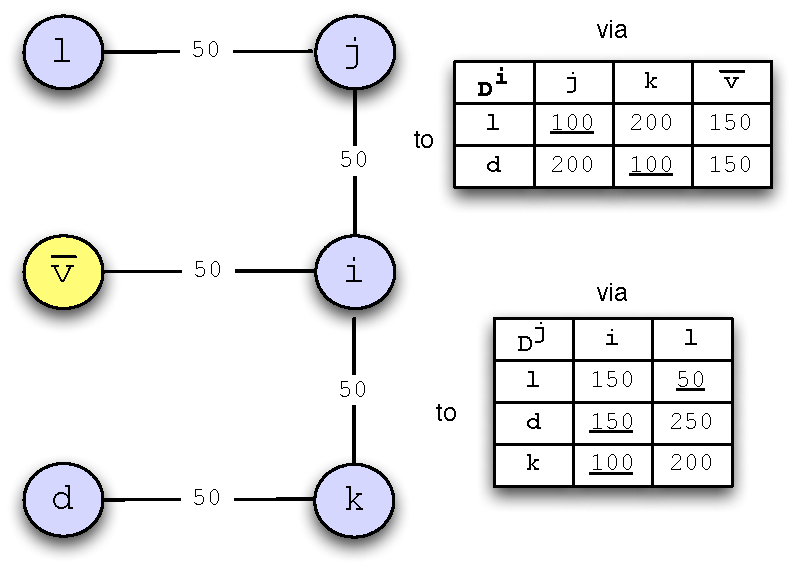
\includegraphics[scale=0.55]{figs/example-a-color.pdf}}
    \subfigure[After $\overline{v}$ is compromised. The dashed lines mark false paths claimed by $\overline{v}$.]
	{\label{fig:example-b}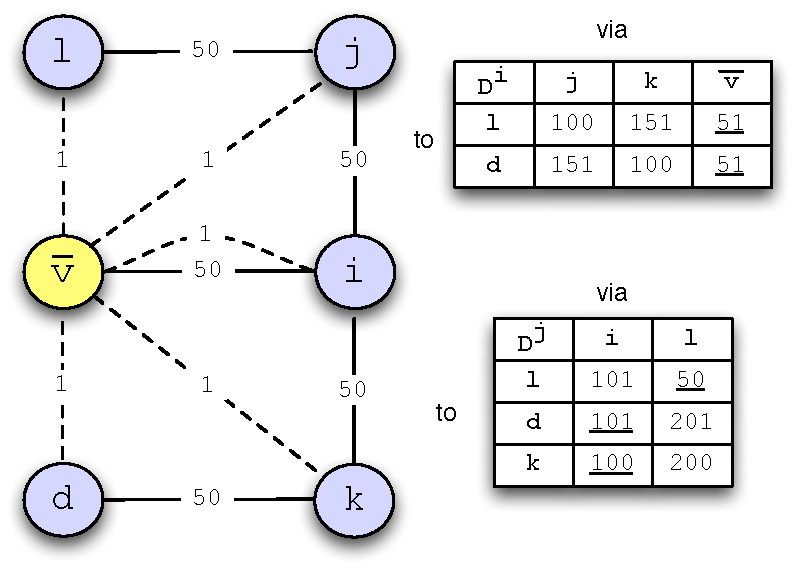
\includegraphics[scale=0.55]{figs/example-b-color.pdf}} 
    \subfigure[After recovery.]{\label{fig:example-c}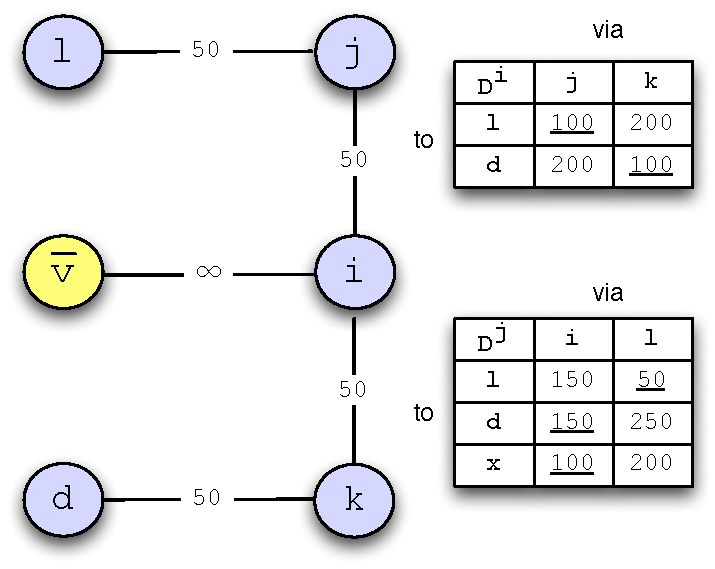
\includegraphics[scale=0.55]{figs/example-c-color.pdf}}
  \end{center}
	%\caption{Three snapshots of a graph, $G$.}
	\caption{Three snapshots of a graph, $G$, where $\overline{v}$ is the compromised node. Parts of $i$ and $j$'s distance matrix are displayed to the right of each sub-figure.
	The least cost values are underlined.}
	%$dmatrix_i$ and $dmatrix_j$ are displayed to the right of each sub-figure.
	%The least cost values are underlined.}
	%(a) $G$  before $\overline{v}$ is compromised, (b) $G$ after $\overrightarrow{bad}$ has}
	%has finished propagating but before recovery has started, and (c) $G$ after recovery. The dashed lines in (b) mark false paths used by $\overrightarrow{bad}$. 
	%Parts of $dmatrix_i$ and $dmatrix_j$ are displayed to the right of each sub-figure. The least cost values are underlined.}
  \label{fig:dv-example}
\end{figure*}


We trace the execution of \second using the example in Figure \ref{fig:dv-example}.
In Figure \ref{fig:example-b}, $i$ uses \bad to reach nodes $l$ and $d$.  $j$ uses $i$ to reach all nodes except $l$.  Notice that when $j$ uses $i$ to reach $d$, 
it transitively uses \badvector (e.g., uses path $j-i-$\bads$-d$ to $d$). 
After the preprocessing completes, $i$ selects a new neighbor to route through to reach $l$ and $d$ by finding its new smallest distance in \dmatrixi 
to these destinations: $i$ selects the routes via $j$ to $l$ with a cost of $100$ and $i$ picks the route via $k$ to reach $d$ with cost of $100$. 
(No changes are required to route to $j$ and $k$ because $i$ uses its direct link to these two nodes). 
Then, using traditional distance vector $i$ sends \minvi to $j$ and $k$.  When $j$ receives \minvis, $j$ must modify its distance to $d$ because \minvi indicates 
that $i$'s least cost to $d$ is now $100$.
$j$'s new distance value to $d$ becomes $150$, using the path $j-i-k-l$. $j$ then sends a message sharing \minvj with its neighbors.  From this point, recovery proceeds according 
by using traditional distance vector. 

%{\bf Pros/Cons.} 
\second is simple and makes no synchronization assumptions. % The primary advantage of \second is its simplicity.
However, \second is vulnerable to the \infinity problem. Because each node only has local information, the new shortest paths may continue to use \bads.
%When computing new shortest paths, a node cannot guarantee that the new shortest path does not use \bad because the node only has local information. 
For example, if $w(k,d)=400$ in Figure \ref{fig:dv-example}, a \infinity scenario would arise. After notification of \bads's compromise, 
$i$ would select the route via $j$ to reach $d$ with cost $151$ (by consulting \dmatrixis), using a path that does not actually exist in $G$ ($i-j-i-$\bads$-d$), since $j$ has removed \bad as a 
neighbor. When $i$ sends \minvi to $j$, $j$ selects the route via $i$
to $d$ with cost $201$. Again, the path $j-i-j-i-$\bads$-d$ does not exist.  In the next iteration, $i$ 
picks the route via $j$ having a cost of $251$. This process continues until each node finds their 
correct least cost to $d$.  We will see in our simulation study that the \infinity problem can incur significant message and time costs.




\subsection{The purge Algorithm}
\label{subsec:purge}


\purge globally invalidates all false state using a diffusing computation and then uses distance vector to compute new distance values that avoid all invalidated paths.
Recall that diffusing computations preserve the decentralized nature of distance vector.
The diffusing computation is initiated at the neighbors of \bad because only these nodes are 
aware if \bad is used an intermediary node. The diffusing computations spread from \bads's neighbors to the network edge, invalidating false state at each node along the way. 
Then ACKs travel back from the network edge to the neighbors of \bads, indicating that the diffusing computation is complete. 
See Algorithm \ref{alg:purge} and \ref{alg:purge2} in the Appendix for a complete specification of this diffusing computation.

Next, \purge uses distance vector to recompute least cost paths invalidated by the diffusing computations.  In order to initiate the distance vector computation, each 
node is required to send a message after diffusing computations complete, even if no new least cost is found.  Without this step, distance vector may not correctly compute new least cost 
paths invalidated by the diffusing computations.  For example, consider the following the scenario when the diffusing computations complete: a node $i$ and all of $i$'s neighbors have 
least cost of $\infty$ to destination node $a$. Without forcing $i$ and its neighbors to send a message after the diffusing computations complete, neither $i$ nor $i$'s neighbors may
never update their least cost to $a$ because they may never receive a non-$\infty$ cost to $a$.

%{\footnote {\small The operations performed by the diffusing compuations described in Section \ref{subsec:preprocess} are  }
%This algorithm is specified in Algorithm \ref{alg:discover} of the Appendix.

In Figure \ref{fig:dv-example}, the diffusing computation executes as follows. First, $i$ sets its distance to $l$ and $d$ to $\infty$ (thereby invalidating $i$'s path to $l$ and $d$)
because $i$ uses \bad to route these nodes. Then, $i$ sends a message to $j$ and $k$ containing $l$ and $d$ as invalidated destinations.
When $j$ receives $i$'s message, $j$ checks if it routes via $i$ to reach $l$ or $d$. Because $j$ uses $i$ to reach $d$, $j$ sets its distance estimate to $d$ to $\infty$. 
$j$ does not modify its least cost to $l$ because $j$ does not route via $i$ to reach $l$. Next, $j$ sends a message that includes $d$ as an invalidated destination.
$l$ performs the same steps as $j$. After this point, the diffusing computation ACKs travel back towards $i$. When $i$ receives an ACK, the diffusing computation is complete. At this
point, $i$ needs to compute new least costs to node $l$ and $d$ because $i$'s distance estimates to these destinations are $\infty$. 
$i$ uses \dmatrixi to select its new route to $l$ (which is via $j$) and uses \dmatrixi to find $i$'s new route to $d$ (which is via $k$). Both new paths have cost $100$. Finally,
$i$ sends \minvi to its neighbors, triggering the execution of distance vector to recompute the remaining distance vectors.

Note that a consequence of the diffusing computation is that not only is all \badvector state deleted, but all \oldvector state as well.  
Consider the case when \bad is detected before node $i$ receives \badvectors.
It is possible that $i$ uses \oldvector to reach a destination, $d$. In this case, the diffusing computation will set $i$'s distance to $d$ to $\infty$.

An advantage of \purge is that it makes no synchronization assumptions. Also, the diffusing computations ensure that the \infinity problem does not occur by removing
false state from the entire network. However, globally invalidating false state can be wasteful if valid alternate paths are locally available. 


\subsection{The cpr Algorithm}
\label{subsec:cpr}

\cprs {\footnote {\small The name is an abbreviation for {\bf C}heck{\bf P}oint and {\bf R}ollback. }} 
is our third and final recovery algorithm. 
Unlike \second and \purges, \cpr only requires that clocks across different
nodes be loosely synchronized i.e. the maximum clock offset between
any two nodes is assumed to be $\delta$. For ease of explanation, we
describe \cpr as if the clocks at different nodes are perfectly
synchronized. Extensions to handle loosely synchronized clocks should
be clear. Accordingly, we assume that all neighbors of \bads, are
notified of the time, $t'$, at which \bad was compromised.

For each node, $i \in G$, \cpr adds a time dimension to \minvi and \dmatrixis, which \cpr then uses to locally archive a complete history of values. 
Once the compromised node is discovered, 
the archive allows the system to rollback to 
a system snapshot from a time before \bad was compromised. From this point, \cpr needs to remove \bad and \oldvector and update stale distance values resulting from link cost changes.
We describe each algorithm step in detail. % (1) Create a \minv and \dmatrix archive. (2) roll back to a valid snapshot, and (3) steps after the rollback. 

{\bf Step 1: Create a \minv and \dmatrix archive.} 
	We define a  \emph{snapshot} of a data structure to be a copy of all current distance values along with a timestamp.
	{\footnote {\small In practice, we only archive distance values that have changed. Thus each distance value is associated with its own timestamp.}}
	The timestamp marks the time at which that set of distance values start being used. 
	\minv and \dmatrix are the only data structures that need to be archived. This approach is similar to ones used in temporal databases 
  \cite{Jensen91,Lomet06}.

  Our distributed archive algorithm is quite simple.  %For a given data structure, a node archives all current distance values whenever one of the values change. 
	Each node has a choice of archiving at a given frequency (e.g., every $m$ timesteps) or after some number of distance value changes (e.g., each time a distance 
	value changes).  Each node must choose the same option, which is specified as an input parameter to \cprs. A node archives independently of all other nodes.
  A side effect of independent archiving, is that even with perfectly synchronized clocks, the union of all snapshots may not constitute a globally consistent snapshot. 
  For example, a link cost change event may only have propagated 
  through part of the network, in which case the snapshot for some nodes will reflect this link cost change (i.e., among nodes that have learned of the event) 
  while for other nodes no local snapshot will reflect the occurrence of this event. We will see that a globally consistent snapshot is not required for correctness.  

{\bf Step 2: Rolling back to a valid snapshot.} 
Rollback is implemented using diffusing computations. Neighbors of the compromised node independently select a snapshot to roll back to, such that the snapshot is the most recent one taken
before $t'$.  Each such node, $i$, rolls back to this snapshot by restoring the \minvi and \dmatrixi values from the snapshot.  Then, $i$ initiates a diffusing computation to inform all other
nodes to do the same. If a node has already rolled back and receives an additional rollback message, it is ignored. 
(Note that this rollback algorithm ensures that no reinstated distance value uses \badvector because every node rolls back to a snapshot 
with a timestamp less that $t'$. ) Algorithm \ref{alg:rollback} in the Appendix gives the pseudo-code for the rollback algorithm.


{\bf Step 3: Steps after rollback.} After Step 2 completes, the algorithm in Section \ref{subsec:preprocess} is executed.
There are two issues to address.
First, some nodes may be using \oldvectors.  Second, some nodes may have stale state as a result of link cost changes that occurred during $[t',t_b]$ and 
consequently are not reflected in the snapshot. 
To resolve these issues, each neighbor, $i$, of \bads, sets its distance to \bad to $\infty$ and then selects new least cost values that avoid the compromised node, triggering
the execution of distance vector to update the remaining distance vectors.  That is, for any destination, $d$, where $i$ routes via \bad to reach $d$,
$i$ uses \dmatrixi to find a new least cost to $d$. If a new least costs value is used, $i$ sends a distance vector message to its neighbors. Otherwise, $i$ sends no message.
Messages sent trigger the execution of distance vector.

During the execution of distance vector, each node uses the most recent link weights of its adjacent links. Thus, 
if the same link changes cost multiple times during  $[t',t_b]$, we ignore all changes but the most recent one. Algorithm \ref{alg:cpr} specifies Step 3 of \cprs.

In the example from Figure \ref{fig:dv-example}, the global state after rolling back is nearly the same as the snapshot depicted in Figure \ref{fig:example-c}:
the only difference between the actual system state and that depicted in Figure \ref{fig:example-c} is that in the former 
$(i,$\bads$)=50$ rather than $\infty$. Step 3 in \cpr makes this change.  Because no nodes use \oldvectors, no other changes take place.

Rather than using an iterative process to remove false state (like in \second and \purges), \cpr does so in one diffusing computation.
However, \cpr incurs storage overhead resulting from periodic snapshots of \minv and \dmatrixs.  Also, after rolling back, stale state may exist if link cost changes occur during $[t',t_b]$.
This can be expensive to update.
Finally, unlike \purge and \seconds, \cpr requires loosely synchronized clocks because without a bound on the clock offset, nodes may rollback to highly inconsistent local snapshots.
Although correct, this would severely degrade \cpr performance.

\subsection{Multiple Compromised Nodes}
\label{subsec:mult}

Here we detail the necessary changes to each of our recovery algorithms when multiple nodes are compromised. Since we make the same changes to all three algorithms, we do not refer 
to a specific algorithm in this section. Let $\overline{V}$ refer to the set of nodes compromised at time $t'$. 

In the case where multiple nodes are simultaneously compromised, each recovery algorithm is modified such that for each $\overline{v} \in \overline{V}$, all $adj(\overline{v})$
are notified that \bad was compromised. 
%to accept a \emph{set} of compromised nodes, $\overline{V}$, as input (rather than a single node).  {\bf not really correct to refer to the set as input}
From this point, the changes to each algorithm are straightforward.  For example,
the diffusing computations described in Section  \ref{subsec:preprocess} are initiated at the neighbor nodes of each node in $\overline{V}$.
{\footnote {\small For \cprs, $t'$ is set to the time the first node is compromised.}}
%First, we augment the preceprocessing procedure described in Section \ref{subsec:preprocess}. In 
%the case where multiple nodes are simulataneously compromised, we modify the diffusing computations to remove all compromised nodes as a destination. %each of these nodes as a destination.

More changes are required to handle the case where an additional node is compromised during the execution of a recovery algorithm. Specifically, when another node is 
compromised, $\overline{v}_2$, we make the following change to the distance vector computation of each recovery algorithm.
{\footnote {\small {Recall that each of our recovery algorithms use distance vector to complete their computation.}} 
If a node, $i$, receives a distance vector message which includes a distance value to destination $\overline{v}_2$, then $i$ ignores said distance value and processes
the remaining distance values (if any exist) to all other destinations (e.g., where $d \neq \overline{v}_2$) normally.  If the message contains no distance information for any 
other destination $d \neq \overline{v}_2$, then $i$ ignores the message.
Because $\overline{v}_2$'s compromise 
triggers a diffusing computation to remove $\overline{v}_2$ as a destination, each node eventually learns the identity of $\overline{v}_2$, thereby allowing the node 
execute the specified changes to distance vector.

Without this change it is possible that the recovery algorithm will not terminate.  Consider the case of two compromised nodes, $\overline{v}_1$ and $\overline{v}_2$,
where $\overline{v}_2$ is compromised during the recovery triggered by $\overline{v}_1$'s compromise.  In this case, two executions of the recovery algorithm are triggered: one when
$\overline{v}_1$ is compromised and the other when $\overline{v}_2$ is compromised.
 Recall that all three recovery algorithms set all link costs to $\overline{v}_1$ to $\infty$ (e.g., $(v_i,\overline{v}_1)=\infty, \forall v_i \in adj(\overline{v}_1)$).
If the first distance vector execution triggered by $\overline{v}_1$'s compromise is not modified to terminate least cost computations to $\overline{v}_2$, the distance vector step of the 
recovery algorithm would never complete because the least cost to $\overline{v}_2$ is $\infty$. 



